\documentclass[class=book, crop=false]{standalone}
\usepackage[subpreambles=true]{standalone}

\usepackage{../../style}

\graphicspath{{./assets/images/}}

\begin{document}
\chapter{Introduzione ai calcolatori}
\section{Un po' di storia dell'informatica}
\paragraph{ENIAC, il primo computer della storia}
Commissionato nel 1946 dal Dipartimento di Difesa degli Stati Uniti, \textbf{ENIAC} (\emph{Electonic Numerical Integrator and Computer}) diventa il primo calcolatore della storia.
Dotato di $18000$ valvole termoioniche, esso occupava una stanza di 9x30 metri, consumando un ammontare spropositato di energia.\\
Il suo impiego principale consisteva nel calcolare traiettorie dei proiettili di artiglieria. Infatti, è doveroso specificare come i primi calcolatori della storia siano stati concepiti per essere sfruttati in applicazioni belliche.

\paragraph{Apollo Guidance Computer}
Prodotto da IBM nel 1969, disponeva di 2800 circuiti integrati, un processore da \unit[0.043]{MHz} e \unit[152]{KByte}  complessivi di memoria ROM/RAM. Presentava un'interfaccia display\&keyboard: i comandi utilizzano una sintassi del tipo "verbo + nome".

\paragraph{Programma 101} Nel 1964 l'Olivetti rilascia il primo \emph{personal computer} della storia, sfortunatamente non avrà successo.

\subsection{Differenziazione dei calcolatori}
Seppur i calcolatori di oggi condividano la stessa idea base, le soluzioni per ciascuna tipologia di applicazione sono piuttosto diverse. A seguire alcuni esempi di diverso tipo di calcolatori:

\begin{table}[H]
	\centering
	\caption{didascalia}
	\subimport{assets/tables/}{table_diff_calcolatori.tex}
\end{table}


Per ovvi motivi, ogni tipologia di calcolatore è meglio adatta per differenti scopi. Ottenere delle buone prestazioni senza eccedere in prezzo e potenza è ciò che decreta il successo commerciale di un prodotto.

\section{Le prestazioni dei calcolatori}
Un buon programmatore, oltre a saper utilizzare degli efficienti paradgmi, deve comprendere la gerarchia di memoria e il concetto di parallelismo: conoscere a fondo il calcolatore è fondamentale.\\
Fino a qualche tempo fa le prestazioni di qualsiasi calcolatore erano in balia della disponibilità di memoria. Al giorno d'oggi invece risulta un problema risolto, tranne per qualche criticità per le applicazioni embedded.\\
Ecco una lista degli elementi che influenzano le prestazioni del calcolatore e il loro ruolo:
\begin{itemize}[noitemsep, nolistsep]
	\item \emph{Algoritmi}: determinano il numero di istruzioni di alto livello e di operazioni di IO.
	\item \emph{Linguaggi di programmazione, compilatori e architetture}: determinano il numero di istruzioni macchina per ogni istruzione di basso livello.
	\item \emph{Processore e sistema di memoria}: determina quanto velocemente è possibile eseguire ciascuna istruzione.
	\item \emph{Sistema di I/O (Hardware e sistema operativo)}: determina quanto velocemente possono essere eseguite le istruzioni.
\end{itemize}

\subsection{La memoria e il processore}
\paragraph*{La memoria}
\`{E} possibile classificare la memoria in:
\begin{itemize}[noitemsep]
	\item \emph{volatile}: è costituita da vari banchi di (tipicamente) 8 chip di RAM dinamica. \`{E} dominata dalle \emph{DRAM}.
	\item \emph{permanente}: è costituita da memorie flash (es. SSD), dischi rigidi e CD/DVD.
\end{itemize}
La prima viene utilizzata per memorizzare dati e programmi mentre vengono eseguiti (per questo motivo viene chiamata anche \emph{memoria principale}): allo spegnimento i dati vengono persi. La seconda viene usata per memorizzare grandi quantità di dati e programmi fra esecuzioni diverse.\\
Il principio di funzionamento dell'hard disk è di magnetizzare delle particelle metalliche distribuite su un substrato:
\begin{itemize}[noitemsep]
	\item I dischi sono organizzati in strutture sovrapposte (cilindri).
	\item Le particelle vengono lette da un dispositivo meccanico (testina) che si sposta radialmente su un braccio (in grado di fare movimenti angolari).
	\item Questa componente rallenta i tempi di accesso ma aumenta al densità di memorizzazione (è possibile arrivare facilmente ai Terabyte).
\end{itemize}

Diversamente dai dischi rigidi elettromeccanici, la memorizzazione su una memoria flash avviene intrappolando una carica elettrica in maniera permanente.\\
I dischi ottici funzionano sul principio di riflessione della luce: viene emesso un raggio laser che viene riflesso dai rilievi, nel caso bit 1, e assorbito dalle buche, nel caso bit 0. Nei dischi riscrivibili è inoltre presente un particolare substrato che se riscaldato torna alla condizione di partenza, eliminando tutti i dati memorizzati.

\paragraph*{Il processore}
La \textbf{CPU} è l'unità centrale di ogni calcolatore. Si compone di:
\begin{itemize}[noitemsep]
	\item \emph{Datapath}: esegue operazioni aritmetiche sui dati.
	\item \emph{Control Unit}: impartisce ordini al datapath, alla memoria e alle componenti IO, sulla base di quanto stabilito dal programma.
\end{itemize}
Il processore offre l'\textbf{ISA} (\emph{Instruction Set Architecture}), un'interfaccia che permette di utilizzarlo senza conoscerne i dettagli. In aggiunta all'ulteriore interfaccia del sistema operativo, insieme formano l'interfaccia binaria delle applicazioni \textbf{ABI} (\emph{Application Binary Interface}). Ciò permette allo sviluppatore di svincolarsi dal livello hardware sottostante, secondo il principio di \emph{astrazione}.\\ Esistono due diversi tipi di architetture ISA:
\begin{itemize}[noitemsep,nolistsep]
	\item \textbf{RISC}: offre un numero ridotto di istruzioni, rivolta soprattutto a sistemi \emph{embedded};
	\item \textbf{CISC}: offre Permette di usufruire di un maggior numero di istruzioni, rivolta prevalentemente ai PC.
\end{itemize}

\subsection{Software di sistema}
Il \emph{sistema operativo}:
\begin{itemize}[noitemsep]
	\item gestisce le operazioni di I/O.
	\item alloca la memoria.
	\item consente il multitasking.
\end{itemize}
Il \emph{compilatore} traduce da linguaggio ad alto livello a linguaggio macchina. Ogni istruzione di quest'ultimo è costituita da una determinata sequenza di \emph{bit}, ossia l'unità di base dell'informazione (1 o 0).\\
L'utilità del compilatore consiste nel facilitare il lavoro del programmatore: non è più necessario implementare il software in codice binario, bensì è possibile utilizzare un linguaggio di programmazione più vicino al linguaggio naturale. Il primo linguaggio sviluppato per questo scopo è stato l'\emph{assembly}. Il software che traduce l'assembly in codice binario si chiama \emph{assembler}.\\
\`{E} possibile riassumere la traduzione di un linguaggio di programmazione di alto livello in codice macchina in due semplici passi:
\begin{enumerate}[noitemsep]
	\item traduzione del linguaggio ad alto livello in linguaggio assembly, per via del compilatore
	\item traduzione del linguaggio assembly in linguaggio macchina, attraverso l'assemblatore.
\end{enumerate}
Spesso fanno eccezione alcuni compilatori che trasformano direttamente il linguaggio ad alto livello in codice macchina.

\subsection{Periferiche di IO}
Il \textbf{mouse} è stato inventato nel 1967 da \emph{Doug Engelbart} nei laboratori della \emph{Xerox}. Attualmente sfrutta la tecnologia ottica: attraverso le variazioni di luce provocate da alcuni led che illuminano il piano, il mouse è in grado di rilevare gli spostamenti.

Gli schermi \textbf{LCD} (\emph{Liquid Crystal Display}) sono costituiti da alcuni cristalli che galleggiano in un fluido: ciascuno di essi corrisponde ad un pixel. Attraverso un campo elettrico è possibile ruotare di 90 gradi ogni singolo cristallo, che di conseguenza può impedire o meno il passaggio della luce secondo il fenomeno fisico della \emph{luce polarizzata}.\\
L'immagine dunque viene rappresentata da una matrice di pixel: ciascuno di essi ha associata una componente rosso, verde, blu (sistema RGB). Questa immagine viene memorizzata in un \emph{frame buffer}, una RAM che viene aggiornata  fino a 100 volte al secondo.

\subsection{Misurazione delle prestazioni}
I moderni processori sono costruiti usando un segnale periodico che ne sincronizza le operazioni. Il \emph{ciclo di clock} è l’intervallo di tempo che intercorre tra due colpi di clock. La frequenza è definita come $\frac{1}{\text{ciclo clock}}$. Il ciclo di clock è misurato in secondi, la frequenza in Hertz.\\

Il tempo necessario per l'esecuzione di un programma dipende da tre fattori:
\begin{itemize}[nolistsep]
	\item il numero di istruzioni dell'algoritmo.
	\item i cicli di clock per istruzione (\emph{CPI}).
	\item la frequenza di clock.
\end{itemize}
\begin{equation*}
\text{Tempo CPU} = \text{Num Istruzioni } \cdot \text{ CPI } \cdot \text{ Periodo Clock} = \frac{\text{Num Istruzioni} \cdot \text{CPI}}{\text{Frequenza Clock}}
\end{equation*}

\begin{figure}[H]
	\centering
	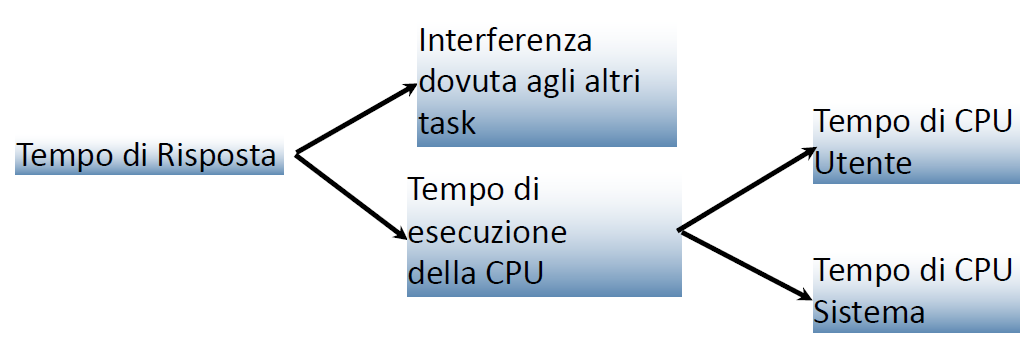
\includegraphics[width=0.9\textwidth,keepaspectratio]{tempo_risposta.png}
	\caption{Diagramma del tempo di risposta}
\end{figure}
Un algoritmo è efficiente se viene strutturato in modo da risparmiare istruzioni e, per una particolare architettura, se utilizza le istruzioni più efficienti (quelle con un basso CPI, poichè il CPI dei diversi tipi di istruzione varia in base all'architettura che deve svolgere le istruzioni).\\
Il linguaggio di programmazione influenza il numero di istruzioni e il CPI: più di alto livello sono i costrutti, più lunghe sono le sequenze di istruzioni macchina ottenute traducendo il codice di partenza.\\
Il compilatore sicuramente influenza sia il numero di istruzioni che il CPI in base alla propria efficienza e ottimizzazione.\\
Anche l'\emph{ISA} ha impatto sul numero di istruzioni, sul CPI, e sulla frequenza di clock attraverso la sua progettazione: essa può fornire istruzioni di basso o alto livello (più o meno istruzioni per eseguire un'operazione).

\subsection{La legge di Moore}
Negli scorsi anni le prestazioni dei calcolatori sono aumentati costantemente, secondo l'andamento previsto da \emph{Moore} attraverso una legge informale.\\
Di recente si è assistito a una diminuzione dell’incremento tra una generazione e l’altra, sintomo di una evidente saturazione, casuata da limiti fisici della materia.

\subsection{La barriera dell'energia}
Dagli anni Ottanta ad oggi, la frequenza media dei processori è stata aumentata di più di mille volte, con conseguente aumento dei consumi di 30 volte.
\begin{equation*}
\text{Potenza} = \text{capacità}\cdot \text{tensione}^2\cdot \text{frequenza di commutazione}
\end{equation*}
Dove la frequenza di commutazione è legata alla frequenza di clock.\\
Incrementare la frequenza senza eccedere in consumi è stato permesso grazie un abbassamento della tensione di alimentazione (termine quadratico, quindi il più influente) da \unit[5]{V} a \unit[1.2]{V}. Al di sotto di questo valore avvengono fenomeni di tipo elettrostatico che portano il sistema in una condizione anomala.\\
C’è inoltre un limite alla capacità di estrarre la potenza prodotta dai processori (e il conseguente calore) tramite ventole o radiatori. Il processo di refrigerazione diventa molto
costoso e difficilmente attuabile in dispositivi desktop e laptop.\\

La soluzione principale che è stata adottata consiste nelle \emph{architetture multicore} sfruttando il concetto di \emph{parallelismo}. Ciò comporta una maggiore difficoltà e responsabilità nella scrittura di codice da parte del programmatore (debugging complicato, bilanciare il carico di lavoro fra le CPU).
\end{document}
